% Chapter Template

\chapter{Arbitrage Theory in Continuous Time Finance} % Main chapter title

\label{Chapter2} % Change X to a consecutive number; for referencing this chapter elsewhere, use \ref{ChapterX}

Arbitrage theory in continuous time finance is a field with a lot of technical details from probability theory and stochastic calculus, where we follow the style in \parencite{Hull, finKont} to focus on intuition without going into the whelm of technicalities and proofs. The focus of this chapter is to provide the basic tools and lay the foundations for the pricing methods. The key question is how to price derivatives fairly and hedge the risk imposed by them. The thesis will mainly deal with the former, where the concepts of arbitrage and replication will be important.\\

We begin by introducing the financial markets and key concepts for building a arbitrage-free and complete market model (section \ref{FinMarket}). Then we build a framework for finding the "fair" price, i.e. finding a arbitrage-free and complete model (section \ref{MultiDimModel}). Lastly, we go into specific cases where either a closed form solution exists or numerical methods are needed (section \ref{classicBS} and \ref{AmericanOptions}).

%----------------------------------------------------------------------------------------
%	SECTION 1
%----------------------------------------------------------------------------------------

\section{Financial Markets}\label{FinMarket}
In the financial markets, there are many agents and different types of investments. The classical investment types are bonds and stocks, where the big players in the markets are commercial banks, investment banks, insurance companies, and pension funds. Derivatives provide additional options for investment.\\

A derivative or a contingent claim is a financial instrument depending on an underlying asset(s), where the dependency is specified in the contract. We will focus on contingent claims with one or two underlying stocks, i.e. univariate and bivariate contingent claims, but the techniques developed can easily be extended to other types of derivatives. \\

In a general setting, to find prices of contingent claims we restrict our financial market to d risky assets $\bm{S}(t)=(S_1(t), S_2(t),\ldots, S_d(t))$ and a bank account $S_0(t)$. The probability space $(\Omega, \mathcal{F}, P)$ with a filtration $\mathbb{F}=(\mathcal{F}_t)_{t\geq 0}$ is fundamental for modeling stochastic processes describing asset prices and trading strategies, where, in the thesis, the filtered probability space $(\Omega, \mathcal{F}, \mathbb{F}, P)$ will be implicitly assumed. Intuitively the filtration $\mathcal{F}_t$ is the information observable at time t, where the filtration $\mathbb{F}^{W}$ generated only by the Wiener processes $(W_t)_{0\leq t \leq T}$ will be important for having a complete market.\\

The bank account is assumed to be a strictly positive adapted process $S_0=(S_0 (t))_{t \geq 0}$ and $S_0(0)=1$, where the d risky assets are modeled by a $\mathbb{R}^d$ adapted stochastic process $\bm{S}=(\bm{S}(t))_{t\geq 0}$. The risky assets are stocks where the stocks are assumed positive $S_i(t)\geq 0$ P-a.s for all i and $t\geq 0$ for financial reasons. By using the bank account as numéraire, i.e. dividing the traded asset by the bank account ($\frac{\bm{S}(t)}{S_0 (t)}$), amounts to working with \textit{zero interest}. We assume that our financial market is frictionless.
\theoremstyle{assumption}
\begin{assumption}{\textbf{Frictionless Market: }}\label{EfficientMarket}
We assume the following institutional facts:
\begin{enumerate}
\item[•] Short positions and fractional holdings are allowed
\item[•] There is no bid-ask spread, i.e. selling price is equal to buying price
\item[•] There are no transactions costs, taxes, or margin requirements of trading
\item[•] The market is completely liquid, i.e. it is possible to buy/sell unlimited quantities on the market. You can borrow an unlimited amount from the bank by short selling
\end{enumerate}
\hfill (p. 6 \parencite{finKont})
\end{assumption}
Besides the assumptions in \parencite{finKont}, we assume the market gives the same uniform price for borrowing money. Stocks are fixed stochastic processes exogenously and a priori given. All the assumptions do not reflect real market conditions, but they are mathematically convenient.

%-----------------------------------
%	SUBSECTION 1
%-----------------------------------

\subsection{Contingent Claims}
A contingent claim is a contract on an underlying asset or assets, where the price of the claim is contingent on the price behavior of the underlying asset(s). A bivariate contingent claim refers to the option being dependent on two risky assets\footnote{Similar refers the multivariate contingent claim to that the claim depends on two or more underlying assets}. We investigate stock derivatives with different types of contracts, where we will mainly divide the derivatives into two classes. 
\begin{enumerate}
\item Simple European derivatives
\item Exotic derivatives (e.g. American options)
\end{enumerate}
Simple European options can only be exercised at maturity (time T) and they depend only on one underlying asset. We have a closed form solution for the simple European options (section \ref{BS-price-EuroCall}). The exotic derivatives are a broad class of functions on the underlying asset(s), where you can e.g. have an American option where the holder can exercise from inception to maturity (section \ref{AmericanOptions}) or a contract on several underlying stocks. Examples of simple European derivatives are the European call and put options.

\theoremstyle{definition}
\begin{definition}{\textbf{European Call and Put Options:}}\label{def:CallOptions}
A European call option is an option where the owner has the right to buy the underlying asset to price K at maturity. If the owner of the option chooses to buy the underlying asset, then the option is exercised. The contract function for the European call option is:
\begin{equation*}
\begin{split}
\Phi(S(T))=\max\{S(T)-K, 0\}
\end{split}
\end{equation*}
The put option is the right to sell the underlying asset to price K at maturity, hence the contract function for the European put option is:
\begin{equation*}
\begin{split}
\Phi(S(T))=\max\{K-S(T), 0\}
\end{split}
\end{equation*}
Where S(T) is the price of the underlying asset at maturity and K is the agreed strike price.
\end{definition}

The American option adds the feature to the European option, that you can exercise at anytime between the inception of the contract until maturity (section \ref{AmericanOptions}). The payoff function is the same for the European and American option. The difference between the European and American option lies in the exercise opportunities. Figure \ref{fig:contractfct} illustrates the European call and put options payoff at maturity. 

\begin{figure}[H]
\centering
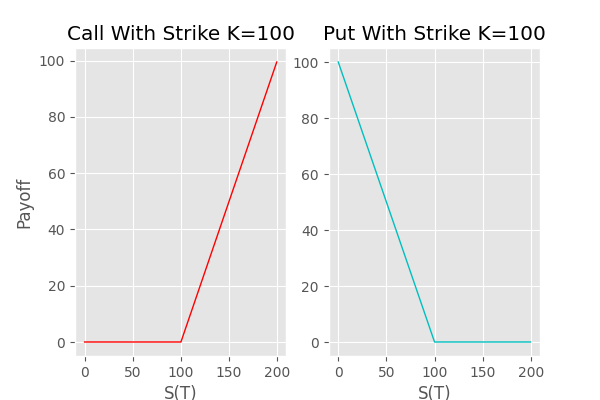
\includegraphics{Figures/contractfct.png}\\
\decoRule
\caption[Contract Functions]{European options payoff at maturity with strike K=100}
\label{fig:contractfct}
\end{figure}

Figure \ref{fig:contractfct} shows that the owner of the option has a limited downside, but the graph does not take into account the initial price for the option. The profit and loss ($P\& L$) graph is also a common way of illustrating the payoff for an option, where the initial cost of buying the option is taking into account. The European call and American put will be the central derivatives considered together with an American bivariate contingent claim. The task ahead is to find the initial price or the fair price for these contracts, where the concepts of completeness and arbitrage will be central.

%-----------------------------------
%	SUBSECTION 2
%-----------------------------------

\subsection{Self-financing Portfolio (Without Consumption)}
Before being able to use the concepts of arbitrage and completeness, the construction of the portfolio from the financial market model will be important. The portfolio is the number of each asset from the market the owner of the portfolio holds. The value of the portfolio for a market model with the bank account and d stocks is:
\begin{equation*}
V^h(t)=\sum_{i=0}^{d} h_{i}(t) S_i(t)
\end{equation*}
$V^h$ is called the value process and $h_i(t)$ is the number of shares of type i during the period "$[t,t+dt)$". For the definition of arbitrage (Definition \ref{Arbitrage}) we need to restrict ourselves to self-financing (S-F) portfolios. A self-financing portfolio h, is a portfolio h which does not get any external injection of money.
\theoremstyle{definition}
\begin{definition}{\textbf{Self-financing portfolio: }}
A portfolio consisting of d+1 asset(s): \\
h(t)=($h_0(t),h_1(t), \dotsc, h_{d}$) is self-financing if:
\begin{equation*}\label{SF}
\begin{split}
dV^{h}(t)=\sum_{i=0}^{d} h_{i}(t) dS_{i}(t)
\end{split}
\end{equation*}
Where $S_{i}$ is the $i'th$ asset in our portfolio.\\ \null \hfill (p. 87 \parencite{finKont})
\end{definition}
When dealing with discrete time finance the S-F portfolio is a budget restriction. This is important intuition for the continuous time version because the continuous time version can be thought of as the limit of the discrete version by letting step sizes in time tending to zero. To avoid pathological effects on the portfolio one often introduces the concept of an admissible portfolio:
\theoremstyle{definition}
\begin{definition}{\textbf{a-admissible portfolio: }}
For some $a\geq 0$, a portfolio h is called a-admissible if its value process $V^h(t)$ is uniformly bounded from below by -a.\\
\null \hfill (p. 139 \parencite{finKont})
\end{definition}
The definition of a-admissible portfolio is to avoid situations as the doubling strategy known from gambling which imposes a limit to the debt arrangement. The important takeaway is that the S-F portfolio is a portfolio where you only reallocate your assets through time within the portfolio.

%-----------------------------------
%	SUBSECTION 3
%-----------------------------------
\subsection{Arbitrage}
Arbitrage is the financial term for a \textsl{"free lunch"}. An arbitrage opportunity produces something out of nothing without risk. For an efficient and well-functioning market the \textsl{"money pumps"} cannot exist for long because the \textsl{"free lunch"} would quickly be eroded by exploitation. To avoid making a \textsl{"money machine"} in our market, we want to price derivatives by not introducing arbitrage to the market.  
\theoremstyle{definition}
\begin{definition}{\textbf{Arbitrage: }}\label{Arbitrage}
An arbitrage possibility on a financial market is an admissible self-financed portfolio h such that
\begin{equation*}
\begin{split}
V^{h}(0)=0\\
P(V^{h}(T)\geq 0)=1\\
P(V^{h}(T)>0)>1
\end{split}
\end{equation*}
The financial market $\bm{S}$ is called arbitrage-free if there exists no arbitrage opportunities.\\
\null \hfill (p. 96 \parencite{finKont})
\end{definition}
From the above definition we see that arbitrage is a natural financial requirement for a financial market model because the investor in an arbitrage portfolio can start with 0 dollars, and without injecting any money, the investor is certain of not losing any money. In addition, he has a positive probability of ending up with more than 0 at maturity. This cannot be a well-functioning market for both buyers and sellers. To price the derivatives fair in the model, the derivative should not introduce arbitrage to the market. An arbitrage-free market is not the only desirable property for the market, we would also like to have a unique price for the derivatives. We can obtain a unique price by replication of the cash flow from the derivative with the other assets in the market model. If every derivative can be replicated the market is complete. 

%-----------------------------------
%	SUBSECTION 4
%-----------------------------------

\subsection{Complete Market and Replication}
The replication argument in Black-Scholes paper \parencite{B-S-Paper} was groundbreaking in the sense that the attitude to risk was irrelevant for pricing because by continuous trading in the underlying asset(s) the cash flow from the contingent claim could be replicated. The replication argument shows that the price is unique under the assumption that investors prefer more to less.\\

Replication is also important for risk management of the derivative books because it tells you how to risk neutralizes your exposure\footnote{Note there is a subtle difference between to hegde or replicate a cash flow. The hedge gives minus the cash flow from replication}. In the definition below, we define a replication for a simple T-claim\footnote{Options only exercisable at maturity}.
\theoremstyle{definition}
\begin{definition}{\textbf{Replication and completeness for T-claim: }}
A T-claim X can be replicated, if there exists a self-financing portfolio h such that:
\begin{enumerate}
\item[•] $V^{h}(T)=X$ P-a.s.
\end{enumerate}
I.e. h is a replication portfolio for X if it is guaranteed to pay in all circumstances an amount identical to the payout of the derivative X.
The market is complete if every derivative in the market can be replicated.\\
\null \hfill (p. 192 \parencite{finKont})
\end{definition}

By introducing the basic concepts for how to price fairly and protect ourselves against financial risk, we will in the next section focus on building the financial market model.

%----------------------------------------------------------------------------------------
%	SECTION 2
%----------------------------------------------------------------------------------------

\section{Multidimensional Models}\label{MultiDimModel}
There are two main methods for building a arbitrage-free and complete market model. The classical approach is the delta hedging approach \parencite{B-S-Paper} and \parencite{CRR}). The more advanced mathematical approach is the martingale approach  \parencite{finKont}. In this section, we focus on the martingale approach and show that the delta hedging approach coincides with the more general martingale theory. For the martingale approach, the First and Second Fundamental Theorems of Mathematical Finance will be the key to obtain a fair market. Besides the financial market assumptions in section \ref{FinMarket} will we assume specific model assumptions.

\subsection{Model Assumptions}
Let us consider a filtered probability space $(\Omega, \mathcal{F}, P, (\mathcal{F}_t^{\bar{W}})_{t \in [0,T]})$. Note the assumption that the filtration is generated from the Wiener process and we consider a finite horizon. We assume $\bar{W}_i$ is k-dimensional and $\bar{W}$ is the only random source. A priori we assume a market $(B(t),S_1(t), S_2(t),\ldots, S_d(t))$, where ${S_i(t)}_{i=1,2,\ldots,d}$ are d risky assets and B(t) is the risk-free asset\footnote{B(t) is often called the bank account}. By assumptions their dynamics are given by:\\
\begin{align}
d\bm{S}(t)&=D[\bm{S}(t)]\bm{\alpha}(t)dt+D[\bm{S}(t)]\bm{\sigma}(t)d\bar{\bm{W}}(t) \quad & S_i(0) &\in \mathbb{R}^+ \label{GBM-P} \\
dB(t)&=r(t)B(t)dt \quad & B(0) &= 1
\end{align}
We assume $\alpha_i(t)$, $\sigma_{ij}(t)$ and the short rate $r(t)$ are adapted and bounded processes, these conditions are necessary for the stochastic integrals to be well-defined. The evolution of the stocks are described by the geometric Brownian motion (GBM) which has a solution to the SDE. The randomness comes from the Wiener process\footnote{A Wiener process is also called a Brownian motion} in the GBM, which has wild trajectories. The function $t\mapsto W(t,\omega)$ from $[0,\infty)$ to $\mathbb{R}$ is continuous but nowhere differentiable. Furthermore, the Wiener process has nonzero quadratic variation and infinite variation, which is the reason for stochastic calculus pioneered by Itô. The Wiener process also has well-behaved property, e.g. it is a Lévy process:
\begin{enumerate}
\item[•] $W(0)=0 \quad a.s$
\item[•] Independent and stationary increments $W(t)-W(s)$ which is normally distributed with mean zero and variance t-s
\item[•] W has continuous trajectories\\
\null \hfill (p. 40 \parencite{finKont})
\end{enumerate}
The Wiener process in the GBM formalizes \textsl{"random shocks"} $dW$ to the stock return with volatility $\bm{\sigma}(t)$ and drift $\bm{\alpha}(t)$. Figure \ref{fig:BM} illustrates three approximations to sample paths of the stocks with GBM assumption and initial value $S_{i}(0)=36$.\\

\begin{figure}[th]
\centering
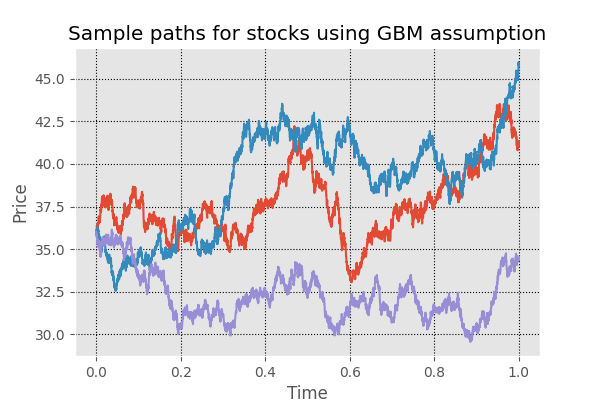
\includegraphics{Figures/samplePath.png}
\decoRule
\caption[Sample Path for Stocks]{Three sample paths for a stock under GBM assumption, where the spot is \$36, $\sigma$=0.2, and $\alpha$=0.06}
\label{fig:BM}
\end{figure}

The tool for handling Wiener processes is stochastic calculus in continuous time because the standard calculus will not work for the wildly behaved Wiener process. In the representation of the GBM, we used vector and matrix notation. The stock vector is d dimensional and the Wiener process vector is k dimensional. The volatility matrix is given by $\bm{\sigma}(t)=\{\sigma_{ij}(t)\}_{i=1,\ldots,d,j=1,\ldots,k}$ and the drift is $\bm{\alpha}(t)=(\alpha_1(t), \alpha_2(t), \ldots, \alpha_d(t))^T$. D(x) denotes a diagonal matrix with vector x as its diagonal and the Wiener processes instantaneous correlation matrix $\Sigma$ is given by $Cov(dW_i(t),dW_j(t))=E(dW_i(t)dW_j(t))=\rho_{ij}dt$.

\subsection{Arbitrage-free Model}
The first problem we are faced with in arbitrage theory is to create a model with no arbitrage opportunities. The First Fundamental Theorem tells us how to not introduce arbitrage to our market model.
\begin{theorem}\label{FFT1}
\textbf{First Fundamental Pricing Theorem of Mathematical Finance(FFT1): } The market model is free of arbitrage if and only if there exists an equivalent martingale measure, i.e. a measure $Q\sim P$ such that the processes:
$$\frac{S_0(t)}{S_0(t)}, \frac{S_1(t)}{S_0(t)}, \cdots, \frac{S_d(t)}{S_0(t)}$$
are (local)martingales under Q.
\\ \null \hfill (p. 154 \parencite{finKont})
\end{theorem}
Assuming $S_0(t)$ is the bank account $B(t)$, then the martingale property for the discounted price processes is a mathematical formulation that the expected discounted value coincides with the known spot value today\footnote{Assuming $B(0)=1$}. In gambling, a martingale resembles a \textsl{"fair"} game. From the FFT1 using the bank account $B(t)$ as numéraire, it follows that:
\theoremstyle{proposition}
\begin{proposition}{}
We assume that $B(t)=S_0(t)$ is our numéraire and all the processes' randomness comes from the Weiner process, then an equivalent measure $Q \sim P$ is a martingale measure if and only if all assets $(B(t), S_1(t), \ldots, S_d(t))$ have the short rate as their local rates of return, i.e.
\begin{align*}
dS_i(t)=S_i(t)r(t)dt+S_i(t)\bm{\sigma}_i(t)d\bm{W}(t)
\end{align*}
\null \hfill (p. 154 \parencite{finKont})
\end{proposition}
So, to not introduce arbitrage to the model for the financial market, we need to ensure the Q-dynamics of S is:
\begin{equation}\label{Q-dym}
d\bm{S}(t)=D[\bm{S}(t)]\bm{r}(t)dt+D[\bm{S}(t)]\bm{\sigma}(t)d\bm{W}(t)
\end{equation}
The tool to obtain the dynamics in equation \eqref{Q-dym} is the Girsanov theorem (theorem \ref{Girsanov}). Girsanov theorem is a continuous measure transformation, where, in our model, we want to transform the dynamics given with the objective probability measure P to an equivalent martingale measure Q. By suitable choices of the likelihood process L and setting $dQ=L(T)dP$, then with Girsanov theorem the transformed process is still a Brownian motion:
$$d\bm{\bar{W}}(t)=\bm{\phi}(t)dt + d\bm{W}(t)$$
When applying to eq. (\ref{GBM-P}):
$$d\bm{S}(t)=D[\bm{S}(t)](\bm{\alpha}(t)+\bm{\sigma}(t)\bm{\phi}(t))dt+D[\bm{S}(t)]\bm{\sigma}(t)d\bm{W}(t)$$
Going back to the FFT1 and the proposition hereof, we know that Q is a martingale measure if and only if:
\begin{align}\label{marketPriceOfRisk}
\bm{\alpha}(t)+\bm{\sigma}(t)\bm{\phi}(t)=\textbf{r}(t) \quad holds \ with \ probability \ 1 \ for \ each \ t
\end{align}
We disregard pathological models, when doing so, the term \textsl{"generically arbitrage-free"} will be used. 

\theoremstyle{definition}
\begin{definition}{\textbf{Generically arbitrage-free}:}
The model in this section is said to be generically arbitrage-free if it is arbitrage-free for every (sufficiently integrable) choice of $\bm{\alpha}(t)$.
\\ \null \hfill (p. 198 \parencite{finKont})
\end{definition}

Furthermore, we assume enough integrability and we have the following useful result:
\theoremstyle{proposition}
\begin{proposition}{}\label{arbitrageFreeProp}
Disregarding integrability problems the model is generically arbitrage-free if and only if, for each $t\leq T$ and P-a.s. the mapping:
$\bm{\sigma}(t):\mathbb{R}^k \to \mathbb{R}^d$ is surjective, i.e. if and only if the volatility matrix $\bm{\sigma}(t)$ has rank d.
\\ \null \hfill(p. 198 \parencite{finKont})
\end{proposition}
We note that to have an arbitrage-free model, we need $k\geq d$, i.e. have at least as many random sources as the number of risky assets. 

\subsection{Complete model}
Second Fundamental Pricing Theorem is key to obtain a complete market model, i.e. a market model with unique prices where every claim can be hedged.
\begin{theorem}\label{FFT2}
\textbf{Second Fundamental Pricing Theorem of Mathematical Finance(FFT2): } Assuming absence of arbitrage, the market model is complete if and only if the martingale measure $Q$ is unique.
\\ \null \hfill (p. 155 \parencite{finKont})
\end{theorem}
In our Wiener world, we have a unique martingale measure if equation \ref{marketPriceOfRisk} has a unique solution. The proof of proposition \ref{completeProp} will shortly reveal why the Wiener world assumption is required. If we had more random sources e.g. a Poisson process\footnote{The Merton's Mixed Jump-Diffusion Model is an example}, then there is no guarantee that the equivalent measure transformation is of the Girsanov type above. 

\begin{proposition}{}\label{completeProp}
Assume that the model is generically arbitrage-free and that the filtration is defined by:
$$\mathcal{F}_t=\mathcal{F}_t^{\bar{W}} \quad t \in [0,T]$$
Then disregarding integrability problems, the model is complete if and only if k=d and the volatility matrix $\sigma(t)$ is invertible P-a.s. for each $t \leq T$
\begin{proof}
The proof is based on martingale representation theorem \ref{MRT} (MRT) and converse of Girsanov theorem \ref{ConverseGirsanov} which uses MRT, hence the assumption about the only randomness comes from the Wiener process. By the two theorems, we know every equivalent measure transformation is obtained by the Girsanov theorem of the above type. Hence, the martingale measure is unique if and only if the solution to \eqref{marketPriceOfRisk} is unique.                                        
\end{proof}
\null \hfill (p. 200 \parencite{finKont})
\end{proposition}
Intuitively we need one independent traded asset excluding the bank account for every source of randomness (Meta-theorem 8.3.1 \parencite{finKont}). Henceforth we will not distinguish between arbitrage-free and generically arbitrage-free.


\subsection{Pricing and Connection to Classical Approach}
The pricing formula for arbitrage-free market model is the risk neutral valuation formula(RVNF):
\begin{proposition}{\textbf{Risk Neutral Valuation Formula: }}\label{RNVF}
To avoid arbitrage, the derivative $\mathcal{X}$ must be priced according to the formula:
\begin{align}
\Pi(t;\mathcal{X})=S_0(t)E^Q[\frac{\mathcal{X}}{S_0(T)}|\mathcal{F}_t]
\end{align}
Note if we choose our numéraire $S_0(t)=B(t)$ then
\begin{align}
\Pi(t;\mathcal{X})=E^Q[\exp(-\int_t^T r(s) ds) \mathcal{X}|\mathcal{F}_t]
\end{align}
\null \hfill(p. 155 \parencite{finKont})
\end{proposition}
Proposition \ref{RNVF} will raise the question if there is more than one fair price for the derivative. The answer is found in FTT2, the market is complete if and only if the measure Q is unique. The conditional expectation in the RNVF is a natural choice for pricing, because intuitively, the conditional expectation is our best estimate given the available information\footnote{Mathematically known as the projection property}.\\

The classical approach in \parencite{B-S-Paper} to a arbitrage-free and complete market model is based on a Markovian model assumption. For the model to have the Markov property, we assume $k=d$ and the probability space is $(\Omega, \mathcal{F}, P, \mathcal{F}_t^{\bar{W}_t})$. Furthermore, we assume $\bm{\alpha}$ and $\bm{\sigma}$ are deterministic and constant over time. $\bm{\sigma}$ is also assumed invertible. Under these more restrictive assumptions, the risk neutral valuation formula for a simple T-claim is given by the pricing function:
\begin{align}\label{MarkovRNVF}
F(t,\bm{S}(t))=\exp(-r(T-t))E^Q[\mathcal{X}|\bm{S}(t)]
\end{align}
The Markov property implies that the price only depends on the current state of $\bm{S}$. Applying Kolmogorov backward equation on equation \eqref{MarkovRNVF} we obtain the Black-Scholes PDE for the pricing function $F(t,\bm{S}(t))=\Pi(t; \mathcal{X})$.

\begin{theorem}\label{BSPDEMultiDim}
\textbf{Black Scholes PDE: } Consider the contract $\mathcal{X}=\Phi(\bm{S}(T))$. In order not to introduce arbitrage to the market, the pricing function $F(t,s)$ must solve the boundary value problem.
\begin{equation*}
\begin{split}
F_t(t,s)+\sum_{i=1}^{d} rs_i \dfrac{\partial F_i(t,s)}{\partial s_i}+\frac{1}{2} \sum_{i,j=1}^{d} s_is_j \frac{\partial F(t,s)}{\partial s_i \partial s_j} (\sigma \sigma^T)_{i,j} -rF(t,s)&=0\\
F(T,s)&=\Phi(s)
\end{split}
\end{equation*}
\null \hfill (p. 203 \parencite{finKont})
\end{theorem}


%----------------------------------------------------------------------------------------
%	SECTION 3
%----------------------------------------------------------------------------------------
\section{Classical Black-Scholes Theory}\label{classicBS}
We will not do the classical delta hedging approach in \parencite{B-S-Paper}. Instead, we use the general multidimensional martingale approach to derive the essential formulas for pricing. 
To derive a closed form solution to the European call and put option, we concentrate on a special case of the multidimensional framework, where we only have the risk-free asset and one risky asset in the financial market model. 
We further restrict ourselves to:
\theoremstyle{assumption}
\begin{assumption}{\textbf{Black-Scholes assumptions}:}\label{BS-Assumption}
We assume the following ideal conditions in addition to \eqref{EfficientMarket}:
\begin{enumerate}
\item[•] The short-term interest rate $r\in \mathbb{R}^+_*$\footnote{Note that restricting the interest rate to the positive reals is not part of the Black-Scholes papers assumptions.}, volatility $\sigma \in \mathbb{R}^+$ and the drift $\alpha\in \mathbb{R}$ are constant.
\item[•] The stock pays no dividends or other distributions.
\item[•] The option is simple ("European").
\item[•] No arbitrage opportunity on the market.
\end{enumerate}
\null \hfill (p. 640 \parencite{B-S-Paper})
\end{assumption}
The interest rate is assumed strictly positive to assure the European call and American call value coincides\footnote{Detailed explained in section \ref{AmericanCall}}. The above assumptions gives the Markovian model described in the previous section. \\

We assume the underlying stock and the bank account have differentials:
\begin{align*}
dS(t)&=S(t)\cdot \alpha dt+S(t) \sigma d\bar{W}(t) \quad & S(0) &\in \mathbb{R}^+ \\
dB(t)&=r B(t)dt \quad & B(0) &= 1
\end{align*}
By Itô's lemma (lemma \ref{Ito}) for one dimensional process the solution to the differentials above is:
\begin{align*}
S(t)&=S(0) \cdot \exp \bigg( (\alpha -\frac{1}{2} \sigma^2) t + \sigma W(t) \bigg) \\
B(t)&=\exp(r\cdot t)
\end{align*}
The solution of the SDE of S under Q dynamics is:
\begin{equation}\label{GBM}
\begin{split}
S(t)=S(0) \cdot \exp \bigg( (r -\frac{1}{2} \sigma^2) t + \sigma W(t) \bigg)
\end{split}
\end{equation}
By equation \eqref{GBM} we see that the Black-Scholes model assumes that the stock price evolution produces a lognormal distribution for the price at any future time. \\

The closed form solution for the European call can be derived from solving the Black-Scholes PDE or with the RNVF given in previous section. 
\theoremstyle{proposition}
\begin{proposition}{}\label{BS-price-EuroCall}
\textbf{Black-Scholes formula for a call option: } The price of a European call option with strike K and maturity T is given by the formula  $\Pi(t)=F(t,S(t)$, where
\begin{align*}
F(t,s)=c(t,s)=s \cdot N(d_1(t,s)) - e^{-r(T-t)}\cdot K \cdot N(d_2(t,s))
\end{align*}
N is the cumulative distribution function of a standard normal distribution $\mathcal{N}(0,1)$ and
\begin{align*}
d_1(t,s)=\frac{1}{\sigma\cdot \sqrt{T-t}} \cdot \bigg( \ln(\frac{s}{K}) + (r+\frac{1}{2} \sigma^2) (T-t) \bigg)\\
d_2(t,s)=d_1(s,t)-\sigma \sqrt{T-t}
\end{align*}
\null \hfill (p. 105 \parencite{finKont})
\end{proposition}
We provided only the price for the European call option, but the European put price can readily be obtained by the put-call-parity for European options.

\theoremstyle{proposition}
\begin{proposition}{}\label{put-call-parity}
\textbf{Put-call parity: } 
Assume the call and put option has the same strike price and time to maturity.
\begin{align*}
p(t,s)=K\cdot \exp(-r(T-t))+c(t,s)-s
\end{align*}
\null \hfill (p. 126 \parencite{finKont})
\end{proposition}

The aim of this thesis is to price American put options, but the European option provides a reference price in a closed form. The put-call-parity holds only for European options, where for the American option there is a bound on price difference:
$$S_0 - K \leq C-P \leq S_0 - K \cdot e^{-rT}$$

The above formula for the European call option is the same for an American call option, but is not true for an American put option or call options with underlying stock paying dividends. The result for the American call option was shown by Merton \parencite{Merton73}, that the intrinsic value is never greater than the worth of the option given by the risk-neutral valuation formula. In section \ref{AmericanOptions} we will show a martingale approach to prove the value of a European and American call coincides when the underlying is a non-dividend paying stock.

%----------------------------------------------------------------------------------------
%	SECTION 4
%----------------------------------------------------------------------------------------

\section{American Options and Optimal Stopping}\label{AmericanOptions}
The American options add additional complexity to the pricing problem, because compared to the European option the American option can be exercised at anytime from inception to maturity. The exercise value at time t is also called the intrinsic value of the option. This section is inspired by \parencite{finKont, Shiryaev06,Elliott99} where \parencite{Shiryaev06} is specialized to optimal stopping problems and the two other references provide the fundamentals for option and arbitrage theory in general.\\

We still assume a diffusion setting that the underlying stochastic process for the stock behaves under the risk neutral measure as a GBM. The exercise feature of the American option raises the problem of rationally finding the optimal stopping time to maximize profit. We will assume a finite horizon $T\in \mathbb{R}_*^+$ throughout the thesis, because all the derivatives will be priced in a finite timeframe. Let the gain function $G:\mathbb{R}\to \mathbb{R}$ be a measurable function satisfying:
\begin{equation}\label{existAmer}
E_{x}[\sup_{0\leq t \leq T}|G(S(t))|] < \infty
\end{equation}
where $S$ is the underlying stochastic process. If the integrability condition is satisfied on a finite interval $[0,T]$ (equation \eqref{existAmer}) then the optimal stopping problem for gain function G and $x \in \mathbb{R}$ is well defined. We assumed that the underlying stochastic S(t) process is time-homogeneous, but the assumption can be relaxed. If S(t) is a time-inhomegenous we can extend the underlying process S(t) by time, albeit increasing the underlying process dimension\footnote{This trick is seen in life insurance for models with state duration, where you include the duration process}. We define the optimal value process in terms of the gain process.

\theoremstyle{definition}
\begin{definition}{}\label{optValFunc}
For fixed $(t,x)\in [0,T] \times \mathbb{R}$, and each stopping time $\tau$ with $\tau\geq t$ the optimal value function $V(t,x)$ is defined by
\begin{align}
V(t,x)= \sup_{\tau \in \mathcal{T}^T} E_{t,x}[G(S(\tau))]
\end{align}
A stopping time that realizes supremum for V is called optimal and denoted $\hat{\tau}$.
\\ \null \hfill (p. 341 \parencite{finKont})
\end{definition}

The solution to the optimal stopping problem $\hat{\tau}$ is where supremum is attained and the price is then $V(t,x)$ for $(t,x)\in [0,T] \times \mathbb{R}$. The supremum is taken over all stopping times with respect to the natural filtration $\mathcal{F}_{t}$ belonging in the class of stopping times:
$$\mathcal{T}_0^T=\mathcal{T}^T=\{\tau : 0 \leq \tau \leq T \}$$
The definition of a stopping time $\tau$ can be seen in definition \ref{StoppingTime}. The intuition is that the stopping time is a random time, where we know, at the present time, whether the process is stopped or not. To solve the optimal stopping problem some trivial solutions are immediate by martingale properties:
\begin{proposition}\label{TrivialMG}
The following holds:
\begin{enumerate}
\item[•] If $G(S(t))$ is a submartingale, then it is not optimal to stop at all and $\tau^*=T$
\item[•] If $G(S(t))$ is a martingale, then all stopping times $\tau\in [0,T]$ are optimal
\item[•] If $G(S(t))$ is a supermartingale, then it is optimal to stop immediately. i.e. $\tau^*=0$
\end{enumerate}
\null \hfill(p. 330 \parencite{finKont})
\end{proposition}

Examples of optimal stopping problems could be the American call and put options:
\begin{align*}
C(t,x)=\sup_{\tau \in \mathcal{T}_t^T} E^Q[\exp(-r(\tau-t)) (S(\tau)-K)^+|S(t)=x] \quad for \ t\in [0,T] \ and \ x\in\mathbb{R}^+\\
P(t,x)=\sup_{\tau \in \mathcal{T}_t^T} E^Q[\exp(-r(\tau-t)) (K-S(\tau))^+|S(t)=x] \quad for \ t\in [0,T] \ and \ x\in\mathbb{R}^+
\end{align*}


\subsection{American Call without Dividends}\label{AmericanCall}
The American call option is a special case, because the optimal stopping time is always at the maturity of the options. With martingale machinery, this means the gain function is a submartingale which implies that $\hat{\tau}=T$ (proposition \ref{TrivialMG}). Remember the optimal stopping problem for an American call option:
$$C(t,x)=\sup_{\tau \in \mathcal{T}_0^{T-t}} E_{t,x}^Q[\exp(-r\tau) (S(t+\tau)-K)^+]$$
Looking at the gain function:
\begin{equation*}
\exp(-r t) (S(t)-K)^+ = (\exp(-r t) S_{t} - \exp(-r t) K)^+
\end{equation*}
Recall that the discounted price process $\exp(-r\cdot t) \cdot S_t$ is a Q-martingale and $\exp(-r\cdot t) \cdot K$ is a deterministic decreasing function in t if $r>0$. Furthermore, the function $x \mapsto (x)^+$ is convex and increasing, hence the gain function is a $Q$-submartingale. The last result used is that a convex and increasing function on a submartingale is still a submartingale, hence the optimal stopping time is $\hat{\tau}=T$ if $r>0$.

\subsection{American Put}\label{americanPut}
The arbitrage-free price for an American put at time t:
\begin{equation}\label{AmericanPutPrice}
P(x,t)=\sup_{\tau \in \mathcal{T}_t^T} E^Q[\exp(-r(\tau-t)) (K-S(\tau))^+|S(t)=x] \quad for \ t\in [0,T] \ and \ x\in\mathbb{R}^+
\end{equation}
For the American put, we need computational methods because the American and European put do not coincide as for the call option.

\begin{proposition}{}
Consider the European put and American put options with same maturity T and strike K. If the risk-free rate $r\in \mathbb{R}_*^+$, then for any $t<T$
\begin{equation}
\begin{split}
p(x,t)<P(x,t)
\end{split}
\end{equation}
\begin{proof}
WLOG\footnote{Without loss of generality} we assume that t=0. Define the stopping time
$$\tau = min \{t\geq 0 : S(t) \leq K\bigg(1-\exp\Big(-r\cdot (T-t)\Big)\bigg)\}$$
We consider an exercise strategy $min\{\tau, T\}$, where the strategy is not necessarily optimal. We consider two events:
\begin{enumerate}
\item[1)] $\tau<T$
\item[2)] $\tau \geq T$
\end{enumerate}
The first case is to exercise at time $\tau$ when $S(\tau) \leq K(1-\exp(-r\cdot (T-\tau)))$. Here the payoff by exercising will be at least $K\exp(-r\cdot (T-\tau))$. The cash flow received is then invested into the bank account at time $\tau$. At maturity, the strategy gives the holder of the put a payoff K, where the European contract with strike K will pay less, because the stock price at maturity will be $S(T)>0 \ a.s.$\\

The second case is trivial, because the European and American put will give the same payoff. Since the first case has a positive probability, the American put has a higher discounted expected payoff by following the above strategy regardless of the spot price for the stock. 
\end{proof}
\end{proposition}
The above proposition shows that the optimal stopping strategy is not always to hold the option to maturity, hence the theory of optimal stopping is important for the pricing of American put options. The American put has consequently no closed form solution, but we can search for a lower exercise boundary b(t) such that the holder of the option should exercise when:
$$S(\tau)\leq b(\tau) \quad \tau \leq T$$
The continuation set $C$ and stopping set $\bar{D}$ are given for an American put.
\begin{align*}
C=\{(t,x) \in [0,T) \times (0,\infty) : P(t,x) > G(x) \}\\
\bar{D}=\{(t,x) \in [0,T) \times (0,\infty) : P(t,x) = G(x) \}
\end{align*} 

Hence the first optimal stopping time after time t for the American put is
\begin{equation*}
\begin{split}
\hat{\tau}= \inf\{u \in [t,T] : P(S(u),u) = (K-S(u))^+ \}
\end{split}
\end{equation*}

\subsection{Discrete Time Valuation}\label{DiscreteValueFramework}
To solve the optimal stopping problem numerical methods are required for the American put option. Hence, the first step is to discretize exercise dates. In chapter \ref{Chapter3} we show two approaches to price an American put option, where both are based on calculating the expected continuation value. \\

Suppose the probability space $(\Omega, \mathcal{F}, P)$ is equipped with the natural discrete filtration $(\mathcal{F}_{t_n})_{n=0,1,\ldots,N}$ modeling a financial market. By discretization of time we are actually looking at a Bermudan option, but for sufficient small time steps the Bermudan option approximates the American option well. The tenor structure\footnote{The tenor of an option is the remaining life of the option from today to maturity} is that the time to maturity is divided into a grid of N+1 equidistant points in time $0=t_0\leq t_1\leq t_2, \cdots \leq t_N=T$, where $\Delta t_n = t_n-t_{n-1}=T/N$ for each $n=1, \ldots, N$. A Bermudan option initialized at time $t_0$ has $\mathcal{T}(t_0,t_1,\ldots,t_N)$ exercise dates or decision points, where the option holder chooses to exercise or keep the option alive. \\

The underlying process is assumed to be Markovian with state variables $(S(t_n))_{n=0,1,\ldots,N}$ recording all necessary information about relevant financial variables adapted to the natural filtration in order to solve the optimal stopping problem with the dynamic programming principle. Furthermore, the gain process is adapted to the filtration and square integrable $E[\max_{0\leq n \leq N} |G(S(t_n))|^2]<\infty$, which is a necessary condition for using regression (section \ref{LSM}).\\

The optimal stopping problem in discrete time is to find:
\begin{equation}\label{Bermudanstop1}
\sup_{\tau \in \mathcal{T}(0,1,\ldots,T)} E^Q[G(S(\tau))]
\end{equation}
For using the programmable dynamic programming principle the Snell envelope $(U(t_{n}))_{n=0,1,\ldots, N}$ (definition \ref{snellEnvelope}) of the gain function $G(S(t_n))_{n=0,\ldots,N}$ is useful and defined by:
$$U(t_n)=\esssup_{\tau \in \mathcal{T}(n,\ldots, N)} E^Q[G(S(\tau))|S(t_n)] \quad n=0,1, \ldots, N$$
The Snell envelope $U(t_n)$ is the smallest supermartingale of the gain process $\{G(S(t_n))\}$, i.e. the smallest supermartingale dominating the gain process. Using the Snell envelope theory the optimal stopping problem can be solved with the dynamic programming principle.
\begin{equation}\label{valueIteration}
\begin{split}
\begin{cases}
          U(t_{N}) = G(S(t_N))\\
          U(t_n) = max\{ G(S(t_n)), E^Q[U(t_{n+1})|S(t_n)])\} \quad for \ n={0,\ldots,N-1} \\ 
\end{cases}
\end{split}
\end{equation}
Where $U(t_n)$ is the discounted option value at time $t_n$ not previously exercised and $G(S(t_n))$ is the discounted exercise value.\\

Equation \eqref{valueIteration} is known as value iteration and indicates that the holder should exercise the first time $G(S(t_n))> E^Q[U(t_{n+1})|S(t_n)]$ to maximize the profit from the option. Therefore, the strategy gives the first optimal stopping time. Note that an optimal stopping time will always exist in discrete time when $T<\infty$, but there is though no guarantee that the stopping time is unique. The value iteration provides the optimal value process of the gain process $G(S(t))$ (theorem \ref{SnellEnvelopeTheorem}). So 
$$U(t_n)=E^Q[G(S(\tau_{t_n})|S(t_n)]$$ with 
$$\tau_{t_n}=\min \{ k \geq n : U(t_k) = G(S(t_k)) \}$$ and 
$$E^Q[U(0)]= \sup_{\tau \in \mathcal{T}(0,\ldots, T)} E^Q[G(S(\tau))]=E^Q[G(S(\hat{\tau}))]$$ 
The optimal stopping problem can also be solved in terms of stopping times instead of using the value process. This alternative dynamic programming recursive equation is called policy iteration.
\begin{equation}\label{policyIteration}
\begin{split}
\begin{cases}
          \tau_{t_N} = t_N\\
          \tau_{t_n} = t_n \cdot 1_{\{G(S(t_n)) \geq E^Q[G(\tau_{t_{n+1}})|S(t_n)])\}} + \tau_{t_{n+1}} \cdot 1_{\{G(S(t_n)) < E^Q[G(\tau_{t_{n+1}})|S(t_n)])\}} \quad for \ n={0,\ldots,N-1} \\ 
\end{cases}
\end{split}
\end{equation}

The first approach in chapter \ref{Chapter3}, the binomial model, uses the idea of dynamic programming. The underlying stochastic process is approximated by a discrete binomial recombining tree, which is ready to work backward in time to calculate both European and American option prices. The American put option can be solved recursively in the binomial model with value iteration: 
\begin{equation}\label{BellmanEq}
\begin{split}
\begin{cases}
          P(t_i) = max\{ (K-S(t_i))^+, \exp(-r\cdot \Delta t) E^Q[P(t_{i+1})|S(t_i)\} \quad for \ i={0,\ldots,N-1} \\
          P(t_N) = (K-S(t_N))^+ 
\end{cases}
\end{split}
\end{equation}

The second approach, Least squares Monte Carlo method (LSM), is to combine dynamic programming and Monte Carlo simulation, but this method uses policy iteration instead of value iteration. The method uses regression to calculate the expected continuation value of simulated paths instead of discretization of the underlying stochastic process. LSM overcomes the challenge with a pure simulation method by using regression, because it provides an effective way to evaluate a series of conditional expectations. Both methods will be explained in details in chapter \ref{Chapter3}.





